\documentclass[12pt]{article}
\usepackage{fontspec}   %加這個就可以設定字體
\usepackage{xeCJK}       %讓中英文字體分開設置
\setmainfont{Times New Roman}
\setCJKmainfont{標楷體} %設定中文為系統上的字型,而英文不去更動,使用原TeX字型
\XeTeXlinebreaklocale "zh"             %這兩行一定要加,中文才能自動換行
\XeTeXlinebreakskip = 0pt plus 1pt     %這兩行一定要加,中文才能自動換行
\usepackage{amsmath, amsthm, amssymb} %引入數學符號的套件,例如實數R、定理Thm...
\usepackage{graphicx}                 %現在, 假設我們要插入 pic.png 這個圖檔, 使用
%\title{我是標題}
%\author{我是作者}
%\date{} %不要日期

\newcommand{\uA}       {\mbox{\boldmath$A$}}
\usepackage{textcomp}
\usepackage{array}
\usepackage{graphicx}
\usepackage{colortbl}
\usepackage{color,xcolor}
\usepackage{listings}
\usepackage{array,booktabs}   %這三個為表格使用的套件
\usepackage{textpos}
\usepackage{float}
\usepackage{listings}

\title{Statistical learning assignment 4- chapter 3}
\author{孫浩哲 \hspace{0.7cm} M072040002}
\date{October 11, 2018}
\begin{document}
\maketitle
\begin{itemize}
\item[4.]\ \\[2ex]
(a)\\[2ex]
The residual sum of square(RSS) for the polynomial regression is lower than another one, because of the polynomial regression may fit the data better.\\[3ex]
(b)\\[2ex]
Contrary to (a), polynomial regression have a higher test RSS because the polynomial model may overfit the data.\\[3ex]
(c)\\[2ex]
The RSS for Polynomial regression is lower than another one.The more flexible model, The lower RSS.\\[3ex]
(d)\\[2ex]
No enough information, because the true relationship is non-linear, We have to see which model is closer than another one real model.
\item[5.]
\begin{align*}
\hat{y_{i}}=x_{i}\hat{\beta}
&=x_{i}\frac{\left(\sum_{i'=1}^{n}x_{i'}y_{i'}\right)}{(\sum_{i'=1}^{n}x_{i'}^2)}\\
&=\frac{\left(\sum_{i'=1}^{n}x_{i}x_{i'}y_{i'}\right)}{(\sum_{i'=1}^{n}x_{i'}^2)}\\
&=\left(\frac{\sum_{i'=1}^{n}x_{i}x_{i'}}{\sum_{i'=1}^{n}x_{i'}^2}\right)y_{i'}
\end{align*}
$\therefore a_{i'}=\left(\frac{\sum_{i'=1}^{n}x_{i}x_{i'}}{\sum_{i'=1}^{n}x_{i'}^2}\right)$
\item[6.]\ \\[2ex]
The simple linear regression :
\hspace{25pt}$$y=\beta_{0}+\beta_{1}x$$
We know that\ $\beta_{0}=\bar{y}-\beta_{1}\bar{x}$, so we can write that:
\begin{align*}
&y=\bar{y}-\beta_{1}\bar{x}+\beta_{1}x\\
\Rightarrow &(y-\bar{y})=\beta_{1}(x-\bar{x})
\end{align*}
No matter what the\ $\beta_{1}$ is, the simple linear model passes through\ $(\bar{x},\bar{y})$
\item[11.]\ \\[2ex]
(a)
\begin{verbatim}
> set.seed(1)
> x=rnorm(100)
> y=2*x+rnorm(100)
> model=lm(y~x)
> summary(model)

Call:
lm(formula = y ~ x)

Residuals:
    Min      1Q  Median      3Q     Max
-1.8768 -0.6138 -0.1395  0.5394  2.3462

Coefficients:
            Estimate Std. Error t value Pr(>|t|)
(Intercept) -0.03769    0.09699  -0.389    0.698
x            1.99894    0.10773  18.556   <2e-16 ***
---
Signif. codes:  0 ‘***’ 0.001 ‘**’ 0.01 ‘*’ 0.05 ‘.’ 0.1 ‘ ’ 1

Residual standard error: 0.9628 on 98 degrees of freedom
Multiple R-squared:  0.7784,	Adjusted R-squared:  0.7762
F-statistic: 344.3 on 1 and 98 DF,  p-value: < 2.2e-16
\end{verbatim}
The\ $p$-value of\ $\beta$ is extremely small and t-statistics is large, so we reject the null hypothesis.\\[3ex]
(b)
\begin{verbatim}
> model2=lm(x~y)
> summary(model2)

Call:
lm(formula = x ~ y)

Residuals:
     Min       1Q   Median       3Q      Max
-0.90848 -0.28101  0.06274  0.24570  0.85736

Coefficients:
            Estimate Std. Error t value Pr(>|t|)
(Intercept)  0.03880    0.04266    0.91    0.365
y            0.38942    0.02099   18.56   <2e-16 ***
---
Signif. codes:  0 ‘***’ 0.001 ‘**’ 0.01 ‘*’ 0.05 ‘.’ 0.1 ‘ ’ 1

Residual standard error: 0.4249 on 98 degrees of freedom
Multiple R-squared:  0.7784,	Adjusted R-squared:  0.7762
F-statistic: 344.3 on 1 and 98 DF,  p-value: < 2.2e-16
\end{verbatim}
The p-value is extremely small and t-statistics is large, even larger than the model which has intercept, so we reject the null hypothesis.\\[3ex]
(c)\\[2ex]
They seem to be the inverse function mutually.\\[3ex]
(d)\\[2ex]
\begin{align*}
\hat{\beta}=\frac{\sum_{i=1}^{n}x_{i}y_{i}}{\sum_{i=1}^{n}x_{i}^2}
\end{align*}
\begin{align*}
t
=\frac{\hat{\beta}}{SE(\hat{\beta})}
&=\frac{\sum_{i=1}^{n}x_{i}y_{i}}{\sum_{i=1}^{n}x_{i}^2}\times\sqrt{\frac{(n-1)\sum_{i'=1}^{n}x_{i'}^2}{\sum_{i=1}^{n}(y_{i}-x_{i}\hat{\beta})^2}}\\
&=\frac{\sqrt{(n-1)\sum_{i=1}^{n}x_{i}^2}\sum_{i=1}^{n}x_{i}y_{i}}{\sqrt{(\sum_{i=1}^{n}x_{i}^2)^2\sum_{i=1}^{n}(y_{i}-x_{i}\hat{\beta})^2}}\\
&=\frac{\sqrt{(n-1)}\sum_{i=1}^{n}x_{i}y_{i}}{\sqrt{\sum_{i=1}^{n}x_{i}^2\sum_{i=1}^{n}(y_{i}^2-2x_{i}y_{i}\hat{\beta}+(x_{i}\hat{\beta})^2)}}\\
&=\frac{\sqrt{(n-1)}\sum_{i=1}^{n}x_{i}y_{i}}{\sqrt{\sum_{i=1}^{n}x_{i}^2\sum_{i=1}^{n}y_{i}^2-\sum_{i=1}^{n}x_{i}^2\hat{\beta}(\sum_{i=1}^{n}2x_{i}y_{i}-x_{i}^2\hat{\beta})}}\\
&=\frac{\sqrt{(n-1)}\sum_{i=1}^{n}x_{i}y_{i}}{\sqrt{\sum_{i=1}^{n}x_{i}^2\sum_{i=1}^{n}y_{i}^2-(\sum_{i=1}^{n}x_{i}y_{i})^2}}
\end{align*}
(e)
\begin{verbatim}
> sqrt(99)*sum(x*y)/sqrt(sum(x^2)*sum(y^2)-(sum(x*y))^2)
[1] 18.72593
> sqrt(99)*sum(y*x)/sqrt(sum(y^2)*sum(x^2)-(sum(y*x))^2)
[1] 18.72593
\end{verbatim}
(f)\\[2ex]
As the program shown in (a) \& (b), we can find that the t-statistic of two models are almost same.
\item[13.]\ \\
(a)(b)(c)
\begin{verbatim}
> {
+ x=rnorm(100)
+ eps=rnorm(100,0,0.5)
+ y=-1+0.5*x+eps
+ length(y)
+ }
[1] 100
\end{verbatim}
$\beta_{0}=-1,\beta_{1}=-0.5$\\[3ex]
(d)\\
\centerline{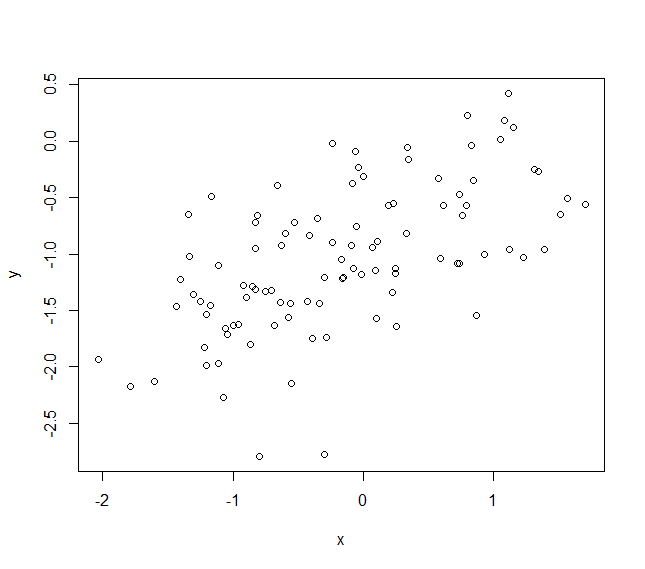
\includegraphics[width=0.8\linewidth]{plot}}
\newpage
(e)
\begin{verbatim}
> {
+ fit=lm(y~x)
+ fit
+ summary(fit)
+ }

Call:
lm(formula = y ~ x)

Residuals:
     Min       1Q   Median       3Q      Max
-1.67217 -0.33359 -0.00624  0.36744  1.05246

Coefficients:
            Estimate Std. Error t value Pr(>|t|)
(Intercept) -0.97000    0.05304 -18.289  < 2e-16 ***
x            0.44834    0.06055   7.405 4.62e-11 ***
---
Signif. codes:  0 ‘***’ 0.001 ‘**’ 0.01 ‘*’ 0.05 ‘.’ 0.1 ‘ ’ 1

Residual standard error: 0.5199 on 98 degrees of freedom
Multiple R-squared:  0.3588,	Adjusted R-squared:  0.3522
F-statistic: 54.83 on 1 and 98 DF,  p-value: 4.62e-11
\end{verbatim}
They are close to the parameter we construct.The\ $p$-value is extremely small, so the null hypothesis can be rejected.\\
\newpage
(f)\\
\raggedright{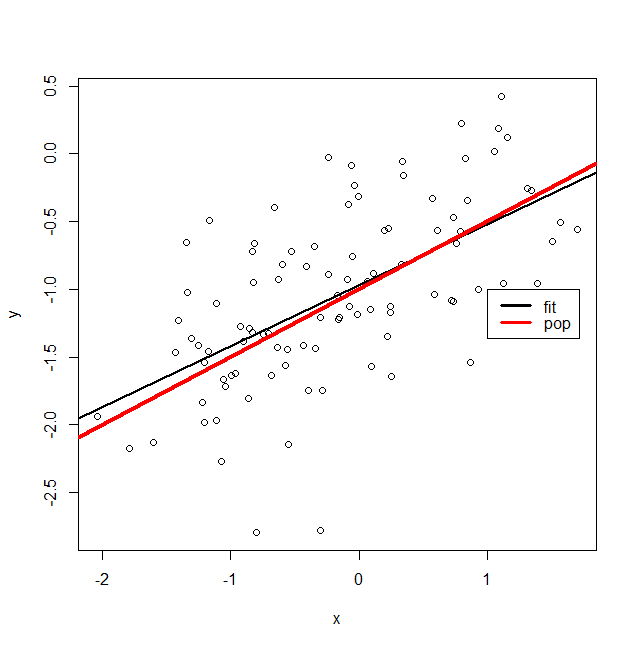
\includegraphics[width=0.8\linewidth]{ab}}\\
(g)\\
\begin{verbatim}
z=x^2
pol=lm(y~x+z)
> summary(pol)

Call:
lm(formula = y ~ x + z)

Residuals:
     Min       1Q   Median       3Q      Max
-1.69645 -0.32512 -0.01374  0.37001  1.02730

Coefficients:
            Estimate Std. Error t value Pr(>|t|)
(Intercept) -0.94408    0.07213 -13.088  < 2e-16 ***
x            0.44327    0.06151   7.206 1.25e-10 ***
z           -0.03493    0.06559  -0.533    0.596
---
Signif. codes:  0 ‘***’ 0.001 ‘**’ 0.01 ‘*’ 0.05 ‘.’ 0.1 ‘ ’ 1

Residual standard error: 0.5218 on 97 degrees of freedom
Multiple R-squared:  0.3606,	Adjusted R-squared:  0.3474
F-statistic: 27.35 on 2 and 97 DF,  p-value: 3.796e-10
\end{verbatim}
The multiple\ $R^2$ of this model is slightly larger than simple linear regression, and the\ $p$-value is also small.\\[3ex]
(h)
\begin{verbatim}
x1=rnorm(100)
eps1=rnorm(100,0,0.1)
y1=-1+0.5*x1+eps1
fit1=lm(y1~x1)
> summary(fit)

Call:
lm(formula = y1 ~ x1)

Residuals:
      Min        1Q    Median        3Q       Max
-0.283441 -0.052967 -0.001256  0.064842  0.271827

Coefficients:
            Estimate Std. Error t value Pr(>|t|)
(Intercept) -0.98516    0.01051  -93.72   <2e-16 ***
x1           0.51626    0.00894   57.75   <2e-16 ***
---
Signif. codes:  0 ‘***’ 0.001 ‘**’ 0.01 ‘*’ 0.05 ‘.’ 0.1 ‘ ’ 1

Residual standard error: 0.1048 on 98 degrees of freedom
Multiple R-squared:  0.9715,	Adjusted R-squared:  0.9712
F-statistic:  3335 on 1 and 98 DF,  p-value: < 2.2e-16
\end{verbatim}
\raggedright{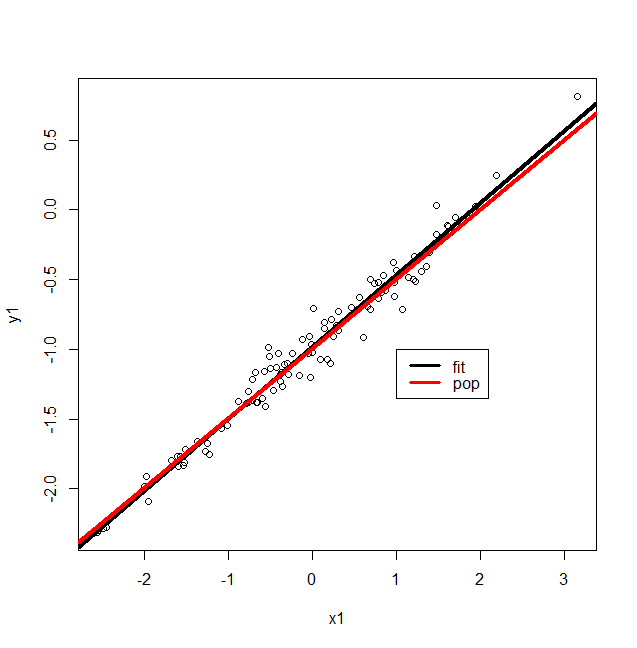
\includegraphics[width=0.7\linewidth]{plot2}}\\
The\ $R^2$ is much larger than the model we build before.\\[3ex]
(i)
\begin{verbatim}
> {
+ x2=rnorm(100)
+ eps2=rnorm(100,0,0.8)
+ y2=-1+0.5*x2+eps2
+ fit2=lm(y2~x2)
+ summary(fit)
+ }

Call:
lm(formula = y2 ~ x2)

Residuals:
     Min       1Q   Median       3Q      Max
-1.95802 -0.41207 -0.03688  0.60361  1.76914

Coefficients:
            Estimate Std. Error t value Pr(>|t|)
(Intercept) -1.02398    0.07849 -13.045  < 2e-16 ***
x2           0.38069    0.07163   5.315 6.71e-07 ***
---
Signif. codes:  0 ‘***’ 0.001 ‘**’ 0.01 ‘*’ 0.05 ‘.’ 0.1 ‘ ’ 1

Residual standard error: 0.7839 on 98 degrees of freedom
Multiple R-squared:  0.2237,	Adjusted R-squared:  0.2158
F-statistic: 28.25 on 1 and 98 DF,  p-value: 6.707e-07
\end{verbatim}
\raggedright{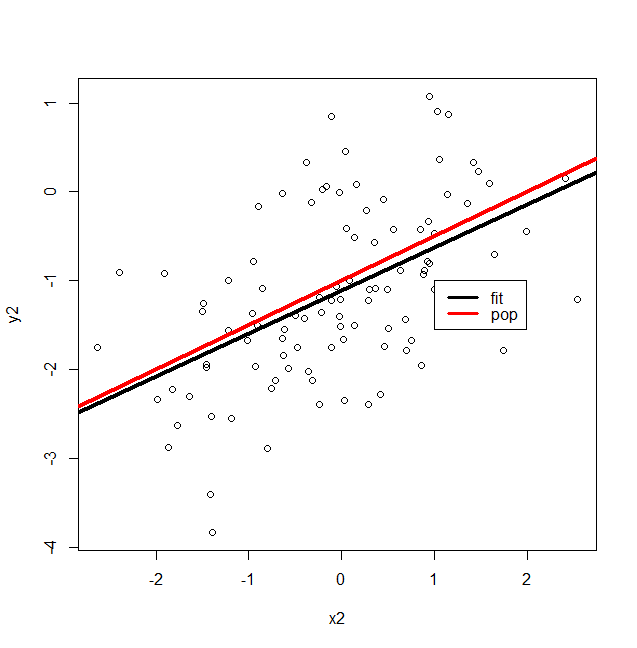
\includegraphics[width=0.7\linewidth]{high}}\\
The\ $R^2$ is smaller than the original model.\\[3ex]
(j)
\begin{verbatim}
> confint(fit)
                 2.5 %     97.5 %
(Intercept) -1.0332352 -0.9710735
x            0.4677338  0.5275863
> confint(fit1)
                 2.5 %     97.5 %
(Intercept) -1.0053096 -0.9932385
x1           0.4880421  0.5001488
> confint(fit2)
                  2.5 %     97.5 %
(Intercept) -1.05712151 -0.9677758
x2          -0.03754376  0.0575819
\end{verbatim}
The more variance we set, the wider confidence interval we get, vice versa.
\end{itemize}
\end{document}